\documentclass[10pt]{article}
\usepackage[utf8]{inputenc}
\usepackage{url}
\usepackage{hyperref}
\usepackage{amsmath}
\usepackage{amsfonts}
\usepackage{amssymb}
\usepackage{graphicx}
\graphicspath{ {./images/} }
\usepackage{float}
\usepackage{lipsum}
\usepackage{sectsty}
\sectionfont{\centering}
\usepackage{multicol}
\usepackage{xcolor}
\usepackage{natbib}
\usepackage{graphicx}
\usepackage{listings}
\usepackage{xcolor}
\usepackage[font=small]{caption}
\addtolength{\abovecaptionskip}{-3mm}
\addtolength{\textfloatsep}{-5mm}
\setlength\columnsep{20pt}

\usepackage[a4paper,left=1.50cm, right=1.50cm, top=2cm, bottom=3cm]{geometry}


\author{}

\title{\Large{Design and Analysis of Algorithms Assignment}}

\begin{document}
	
	\begin{center}
		{\Large \textbf{Design and Analysis of Algorithms Assignment}}\\
		\vspace{1em}
		{\large Department of Information Technology,}\\
		\vspace{1em}
		\large{Indian Institute of Information Technology, Allahabad 211015, India}\\
		\vspace{1em}
		\large{Abhinav(IIT2019098), Harsh Sharma(IIT2019097), Nitesh Rawat(IIT2019099)}
		\vspace{2.5em}
		
	\end{center}
	
\begin{multicols*}{2}

    \textbf{\emph{{Abstract}: Given a string S, count the number of non-empty sub strings that are palindromes. A sub string is any continuous sequence of characters in the string. A string is said to be palindrome, if the reverse of the string is same as itself. Two sub strings are different if they occur at different positions in S.}}\\
	
	\textbf{\emph{{Index Terms}: Arrays, Dynamic Programming, Implementation\\}}


\section*{INTRODUCTION}

We have been given a string S, we have to count the number of palindrome substring in S, A contiguous sequence of characters of a string its called substring. And if the revese of a string is the string itself. It will be called palindrome. Any substring of size 1 will be palindrome obviously, we won't be counting them, we will count the number of palindrome substring whose size is greater than 2. In this paper, we will use the concept of dynamic programming, which has its prime importance, as it reduces the time complexity to a much significant extent.

\paragraph{Dynamic Programming}
Dynamic Programming (DP) is an algorithmic technique for solving an optimization problem by breaking it down into simpler subproblems and utilizing the fact that the optimal solution to the overall problem depends upon the optimal solution to its subproblems. Dynamic Programming is also an optimization over plain recursion. Wherever we see a recursive solution that has repeated calls for same inputs, we can optimize it using Dynamic Programming. The idea is to simply store the results of subproblems, so that we do not have to re-compute them when needed later. This simple optimization reduces time complexities from exponential to polynomial. Dynamic Programmic basically memorizes the answer to the subproblem and use it when necessary.

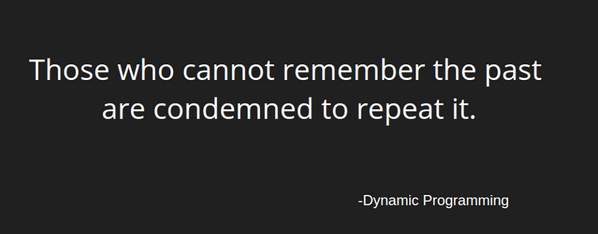
\includegraphics[width=\columnwidth, height=8cm]{DP.png}\begin{center}\textbf{Figure 1:} Dynammic Programming\end{center}


\paragraph{Advantages of Binary Search}
The Dynamic Programming technique generally has following mentioned advantages over Brute Force Algorithms.\\\\
\textbf{Time Efficiency: } This approach generally reduces the running time of the algorithm because the running time of algorithm based on Brute Force is in general high order in nature. But when we are using the approach based on Dynamic Programming, this running time generally decreases because we don't have to calculate the same thing again, as we are storing it already. \\
\\\\\\\\This report further contains:
\begin{itemize}
\item 	Algorithm  Designs
\item 	Algorithm  Analysis
\item 	Experimental Study and Profiling
\item 	Conclusion
\item 	References
\item 	Appendix
\end{itemize}

\section*{ALGORITHM DESIGN}
A general problem based on the dynammic programming. In our paper, we will be following bottom up approach.

\paragraph{Algorithmic Steps:}

In our approach we will create two 2D array, int dp[n][n], and bool P[n][n], where state dp[i][j], will store the number of palindrome from index i to j (i<j), and P[i][j], will store true if substring formed from index i to j is palindrome, else it will store false. Our transition would be, first we update P[i][j], P[i][j] will be true only if P[i+1][j-1] is true and S[i]==S[j], similarly, we would update dp[i][j] to dp[i+1][j]+dp[i][j-1]-dp[i+1][j-1]+P[i][j] (if P[i][j] is true an extra 1 will be added, also we subtract dp[i+1][j-1] to remove the extra part we counted in dp[i+1][j]+dp[i][j-1]).
\begin{enumerate}

\item	Input the string, and store its size in a variable n.
\item	Create two 2D arrays, int dp[n][n] and bool P[n][n];
\item   Initialize p[i][i]= true for all i, and P[i][j]=true and dp[i][j]=1 only if s[i] is equal to s[j], where i=j+1., for any other values in P and dp, we initialize it with false and 0.
\item	Start calculating the values from substring of size 3 to substring of size n, i.e. from gap 2 to gap n-1 between the first and last string of a substring. We set a fixed gap (2 to n-1) in the outer loop.
\item	In the inner loop, We check from each i with a particular gap, i runs from 0 to n-gap-1, and j= i+gap, Update P[i][j] to true, if P[i+1][j-1] is true and s[i] is equal to s[j].Update dp[i][j] to dp[i][j-1]+dp[i+1][j]-dp[i+1][j-1]+P[i][j].
\item	Finally, our answer is stored in dp[0][n-1], we print that.
\\\
\end{enumerate}

\lstset { %
    language=C++,
    backgroundcolor=\color{black!5},
    basicstyle=\footnotesize,
}

\begin{lstlisting}

Int:
Function main()
    string s
    input s
    n = length of s
    dp[n][n] = {0} and P[n][n] = {false}
    for i = 0 to n-1:
        p[i][i] = true
    for i = 0 to n-2:
        if s[i] == s[i+1]:
            dp[i][i+1] = 1
            P[i][i+1] = true
    for gap = 2 to n-1:
        for i = 0 to n-gap-1:
            j = i + gap
            if s[i] == s[j] && p[i+1][j-1]:
                p[i+1][j-1] = true
            dp[i][j] = dp[i][j-1] + dp[i+1][j]
                    - dp[i+1][j-1] + P[i][j]
    
    print dp[0][n-1] //Our answer

\end{lstlisting}
    

	
\section*{ALGORITHM ANALYSIS} 
	
APRIORI ANALYSIS: Let T(n) and S(n) is the time and space respectively with input parameters defined above.

\paragraph{TIME COMPLEXITY DERIVATION:} Let Time complexity of above algorithm be T(n). It is quite intuitive to see that there are two loop, outer loop runs in order of n time and inner loop too runs in order n time, so our time complexity in any case will be O(n^2).
\paragraph{DIFFERENT CASES:} Now let us consider our algorithm in different 
scenarios.\\\\\textbf{BEST CASE/AVERAGE CASE/WORST CASE:} The time and space complexity of our approach in all the three cases is same , i.e, Time Complexity is  O(n^2\)),in any case. Space complexity is the O(n^2\)) in any case because we used two arrays of size n^2.

\section*{PROFILING}

So, after the above analysis, let us have the glimpse of space and time graph and then comparison between both the approaches as a follow-up.

\paragraph{TIME ANALYSIS:}Following is the graph representing the time complexity of the algorithm.\\\\\\
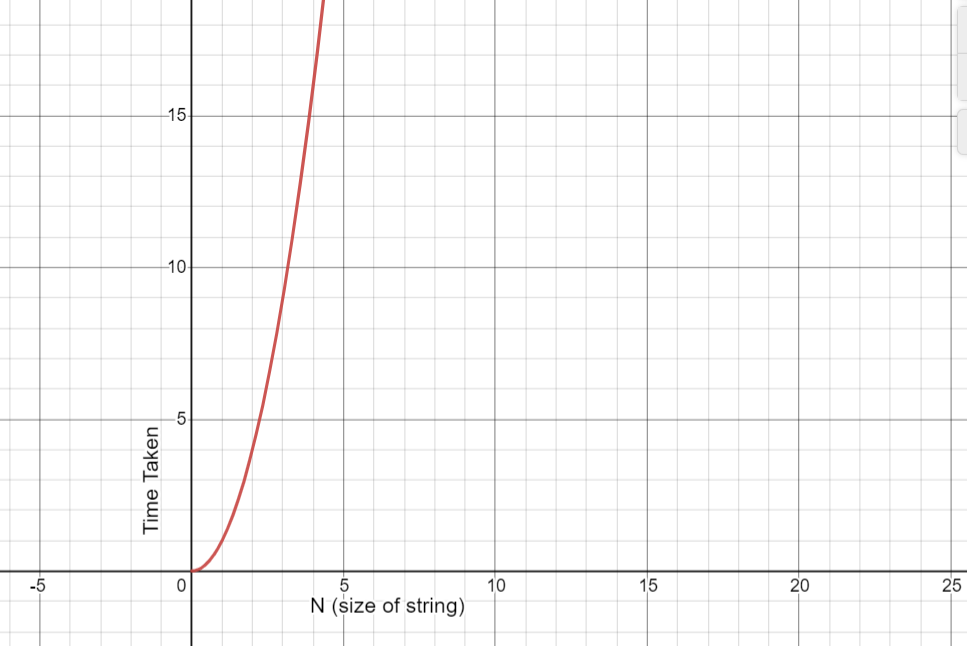
\includegraphics[width=\columnwidth, height=8cm]{Time Complexity.png}\begin{center}\textbf{Figure 2:} Time Complexity Graph\end{center}By the experimental analysis, we found that the more is the value of n, the more time it takes.

\paragraph{SPACE ANALYSIS:}Following is the graph representing the space complexity of the algorithm.\\\\\\
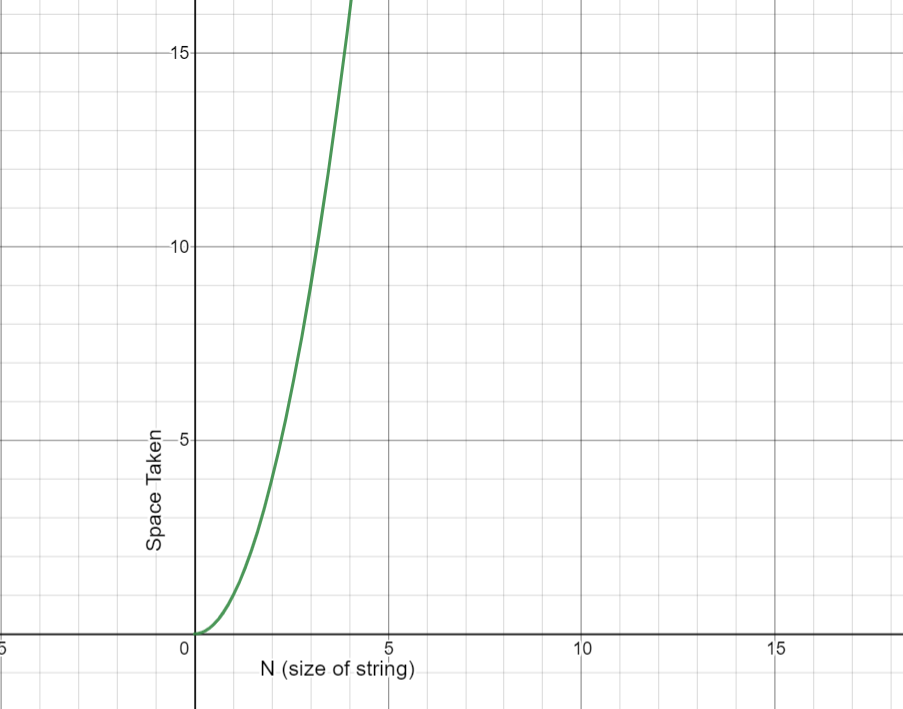
\includegraphics[width=\columnwidth, height=8cm]{Space Complexity.png}\begin{center}\textbf{Figure 3:} Space Complexity Graph\end{center}By the experimental analysis, we found that in any case, space taken is constant.

\section*{APPLICATIONS}
Dynamic programming is both a mathematical optimization method and a computer programming method. The method was developed by Richard Bellman in the 1950s and has found applications in numerous fields, from aerospace engineering to economics. Some of the applications of the Dynamic Programming Approach are:

\begin{enumerate}
\item \textbf{0/1 knapsack Problem:} The knapsack problem is a problem in combinatorial optimization: Given a set of items, each with a weight and a value, determine the number of each item to include in a collection so that the total weight is less than or equal to a given limit and the total value is as large as possible.
\item  \textbf{All pair Shortest path problem:} The Floyd Warshall Algorithm is for solving the All Pairs Shortest Path problem. The problem is to find shortest distances between every pair of vertices in a given edge weighted directed Graph. 
\item \textbf{Longest common subsequence (LCS):} Here we find the longest common subsequence of two strings.
\item \textbf{Sum subset problem:} Given a set of non-negative integers, and a value sum, determine if there is a subset of the given set with sum equal to given sum. We can use dynamic programming even for xor sum subset.
\item \textbf{Maximum subarray sum:} Given an array on integers, we can find a subarray with maximums sum.
\end{enumerate}
\section*{CONCLUSION}

So, with the above mentioned algorithms and their profiling, we come to the conclusion that this problem of finding the number of integers with trailing zeroes equal to n is achieving its best time complexity of O(n^2\)) and space complexity of O(n^2\)).\\ Also, dynamic programming proved to one of the most efficient algorithm here.
Can the algorithm be more improved? Yes, we can do it in linear time and space using Manacher's algorithm.

\section*{ACKNOWLEDGMENT}

We are very much grateful to our Course instructor Dr Mohammed Javed and our mentor, Md Meraz, who have provided the great opportunity to do this wonderful work on the subject of Data Structure and Algorithm Analysis specifically on the programming paradigm of Divide and Conquer.

\section*{REFERENCES}

\begin{enumerate}
\item Introduction to Divide and Conquer Technique:\\
https://www.geeksforgeeks.org/divide-and-conquer-algorithm-introduction/
\item Introduction to Algorithms by Cormen,Charles, Rivest and Stein.\\
https://web.ist.utl.pt/~fabio.ferreira/material/asa
\end{enumerate}
\end{multicols*}

\newpage
\section*{APPENDIX}
\textbf{To run the code, follow the following procedure:}\\
\begin{enumerate}
    \item Download the code(or project zip file) from the github repository.
    \item Extract the zip file downloaded above.
    \item Open the code with any IDE like Sublime Text, VS Code, Atom or some online compilers like GDB.
    \item If required, save the code with your own desirable name and extension is .cpp
    \item Run the code following the proper running commands(vary from IDE to IDE)
    \begin{enumerate}
        \item \textbf{For VS Code:} Press Function+F6 key and provide the input on the terminal.
        \item \textbf{For Sublime Text:} Click on the Run button and provide the input.\\
    \end{enumerate}
\end{enumerate}
\textbf{Code for Implementation is:}
\lstset { %
    language=C++,
    backgroundcolor=\color{black!5},
    basicstyle=\footnotesize,
}

\begin{lstlisting}
#include <bits/stdc++.h>
using namespace std;
int main() {
    string s;
    cin>>s;
    int n=s.size();
    int dp[n][n];
    memset(dp, 0, sizeof(dp));
    bool P[n][n];
    memset(P, false, sizeof(P));
    for (int i = 0; i < n; i++)
        P[i][i] = true;
    for (int i = 0; i < n - 1; i++) {
        if (s[i] == s[i + 1]) {
            P[i][i + 1] = true;
            dp[i][i + 1] = 1;
        }
    }
    for (int gap = 2; gap < n; gap++) {
        for (int i = 0; i < n - gap; i++) {
            int j = gap + i;
            if (s[i] == s[j] && P[i + 1][j - 1])
                P[i][j] = true;
            dp[i][j] = dp[i][j - 1] + dp[i + 1][j] - dp[i + 1][j - 1] + P[i][j];
        }
    }
    cout<<"Number of palindrome substring in \""<<s<<"\" with size greater than 1 are: " << dp[0][n - 1];
}
\end{lstlisting}
\clearpage

	
\end{document}